\documentclass[10pt,twocolumn,letterpaper]{article}

\usepackage{cvpr}
\usepackage{times}
\usepackage{epsfig}
\usepackage{graphicx}
\usepackage{rotating}
\usepackage{multirow}
\usepackage[table]{xcolor}
\usepackage{amsmath}
\usepackage[labelfont={bf,small},font=small]{caption}
\usepackage{amssymb}
\usepackage{pifont}% http://ctan.org/pkg/pifont
\newcommand{\cmark}{\ding{51}}%
\newcommand{\xmark}{\ding{55}}%

\newcommand\crule[3][black]{\textcolor{#1}{\rule{#2}{#3}}}

% Include other packages here, before hyperref.

% If you comment hyperref and then uncomment it, you should delete
% egpaper.aux before re-running latex.  (Or just hit 'q' on the first latex
% run, let it finish, and you should be clear).
\usepackage[pagebackref=true,breaklinks=true,letterpaper=true,colorlinks,bookmarks=false]{hyperref}

% \cvprfinalcopy % *** Uncomment this line for the final submission

\def\cvprPaperID{****} % *** Enter the CVPR Paper ID here
\def\httilde{\mbox{\tt\raisebox{-.5ex}{\symbol{126}}}}

% Pages are numbered in submission mode, and unnumbered in camera-ready
\ifcvprfinal\pagestyle{empty}\fi
\begin{document}

%%%%%%%%% TITLE
\title{AGA : Attribute-Guided Augmentation}

\author{First Author\\
Institution1\\
Institution1 address\\
{\tt\small firstauthor@i1.org}
% For a paper whose authors are all at the same institution,
% omit the following lines up until the closing ``}''.
% Additional authors and addresses can be added with ``\and'',
% just like the second author.
% To save space, use either the email address or home page, not both
\and
Second Author\\
Institution2\\
First line of institution2 address\\
{\tt\small secondauthor@i2.org}
}

\maketitle
%\thispagestyle{empty}

%%%%%%%%% ABSTRACT
\begin{abstract}
We consider the problem of data augmentation, i.e., generating artificial
samples to extend a given corpus of training data. Specifically, we propose
attributed-guided augmentation (AGA) which aims to learn a mapping
that allows to synthesize data such that an attribute of a synthesized sample 
is at a desired value or strength. This is particularly interesting in situations 
where little data with no attribute annotation is is available for learning, but 
we have access to a large external corpus of heavily annotated samples. 
While prior works primarily augment in the space of images,
we propose to perform augmentation in feature space directly.
We implement our approach as a deep encoder-decoder architecture that 
facilitates to learn the synthesis function in an end-to-end manner. 
We demonstrate the utility of our approach on the problem of 
one-shot object recognition in a transfer-learning setting where
we have no prior knowledge of the new categories, except for 
a single training sample.
As external data, we leverage 3D depth and pose information from the 
SUN RGB-D dataset and show that attribute-guided augmentation of
high-level CNN features substantially improves one-shot object recognition 
performance.
\end{abstract}

%%%%%%%%% BODY TEXT
\section{Introduction}
\label{section:introduction}

Convolutional Neural networks~(CNNs), trained on large scale data, have significantly advanced the state-of-the-art 
on traditional vision problems such as object recognition~\cite{Krizhevsky12a,Simonyan14a,Szegedy15a} and 
object detection~\cite{Girshick15a,Ren15a}. Success of these networks is mainly due to their high selectivity 
for semantically meaningful visual concepts, \eg, objects and object parts~\cite{Fergus14a}.
In addition to ensuring good performance on the problem of interest, this property of CNNs also allows 
for {\it transfer\/} of knowledge to several other vision tasks~\cite{Donahue14a,Gong14a,Cimpoi15a,Dixit15a}. 
The object recognition network of~\cite{Krizhevsky12a}, \eg, has been successfully used for object 
detection~\cite{Girshick15a,Ren15a}, scene classification~\cite{Gong14a,Dixit15a}, texture 
classification~\cite{Cimpoi15a} and domain adaptation~\cite{Donahue14a}, using various 
transfer mechanisms. 

\begin{figure}[t!]
\centering{
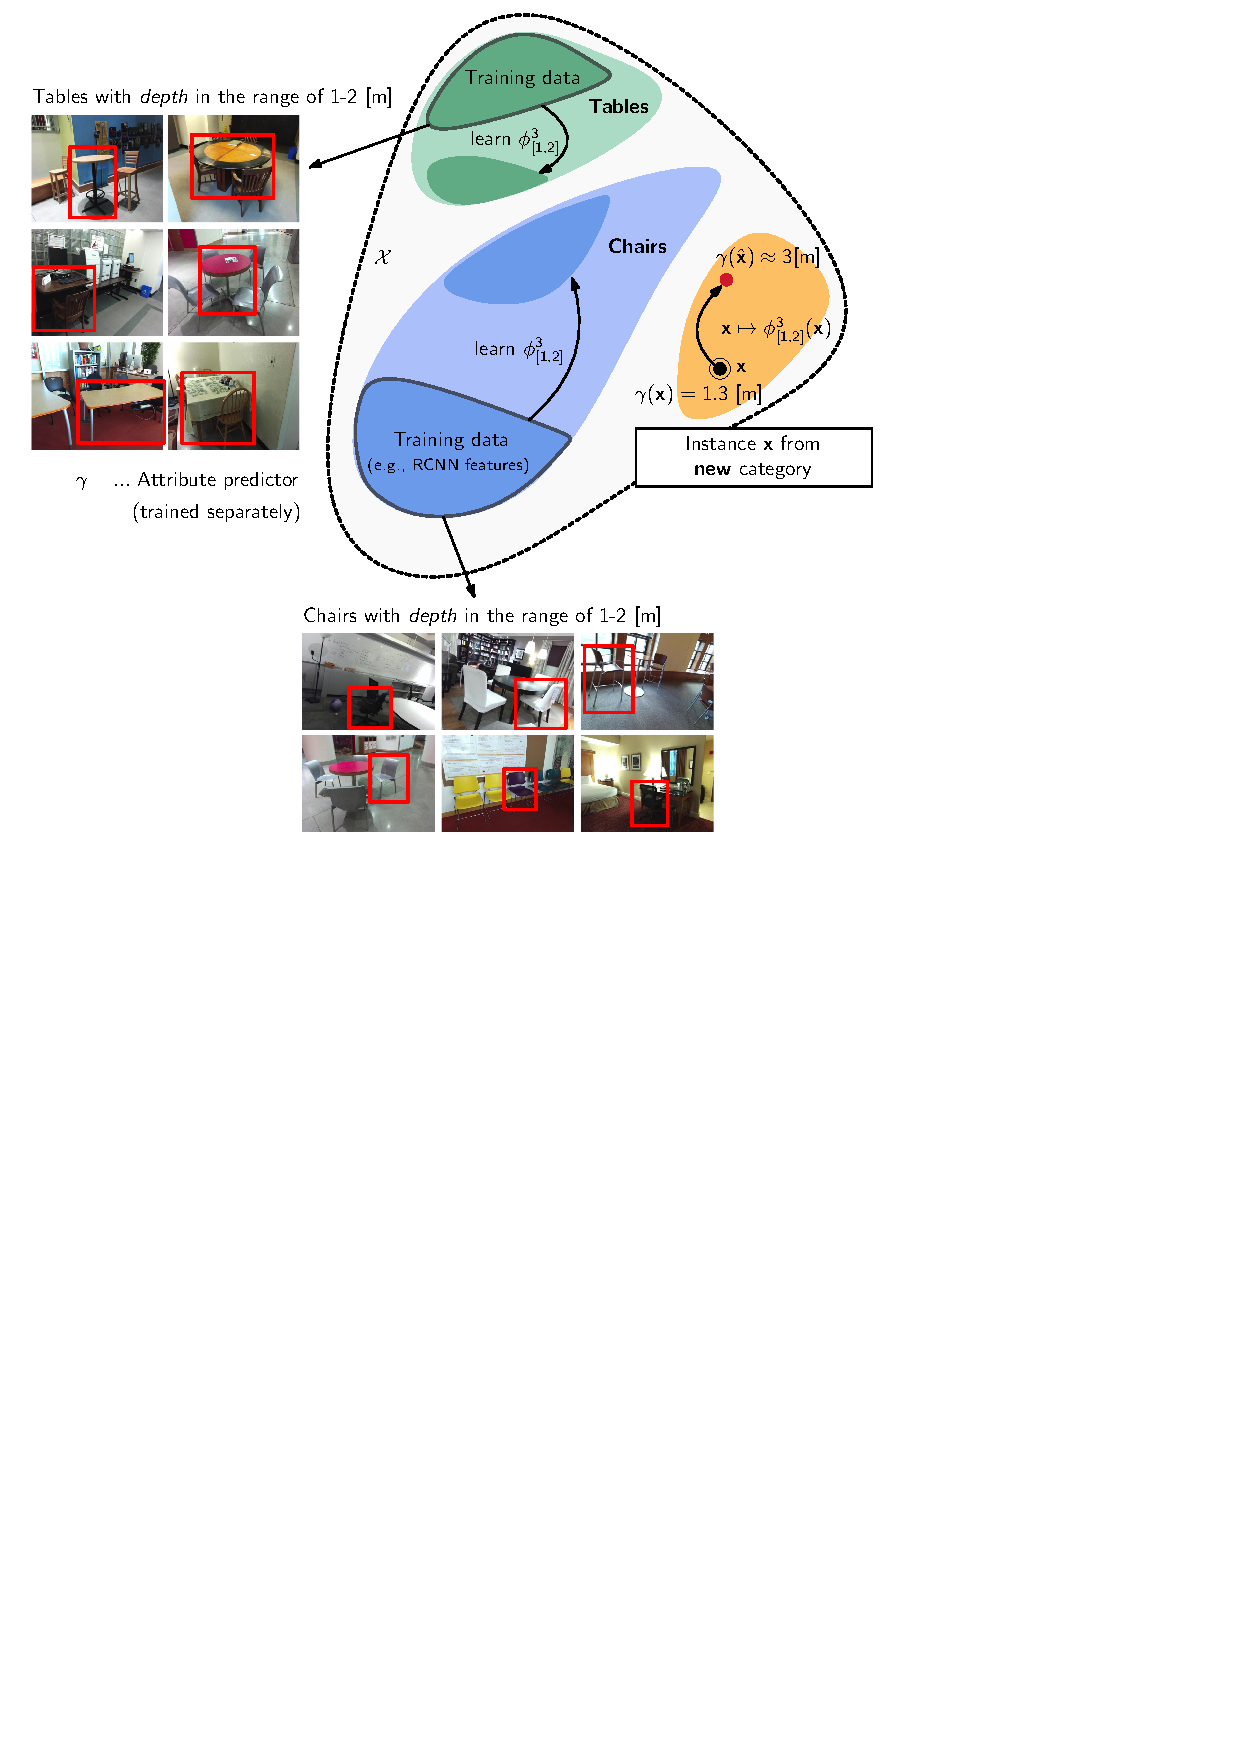
\includegraphics[width=0.99\columnwidth]{figures/Intro2}
}
\caption{\label{fig:intro} Given a predictor $\gamma: \mathcal{X} \to \mathbb{R}_+$ of attribute
strength (\eg, for depth or pose), we propose to \emph{learn} a mapping 
of object features $\mathbf{x} \in \mathcal{X}$, such that
(1) the mapped feature is ``close'' to $\mathbf{x}$ (to preserve object identity) and (2) the predicted 
attribute value $\gamma(\hat{\mathbf{x}}) = \hat{t}$ of mapped features 
$\phi(\mathbf{x}) = \hat{\mathbf{x}}$
matches a given target value $t$. In this example,
we learn a mapping for features with associated \emph{depth} values in the
range of 1-2 [m] to $t=3$~[m] and apply that mapping to an instance of a new 
object category. In our approach, this mapping is learned in 
an \emph{object-agnostic} manner. In our example, this means that
\emph{all} training data from chairs and tables is to learn $\phi$).}
\end{figure}

\vskip1ex
CNN-based transfer is generally achieved either by {\it finetuning\/} a pre-trained network 
such as~\cite{Krizhevsky12a}, on a new image dataset or by designing a new image 
representation on such a dataset with the activations of the pre-trained network 
layers~\cite{Donahue14a,Gong14a,Dixit15a,Cimpoi15a}.
Recent proposals of transfer have shown highly competitive performance on different predictive 
tasks with a modest amount of new data (as few as 50 images per class). The effectiveness 
of transfer based methods, however, has not yet been tested under more severe constrains like 
in a {\it few shot\/} or a {\it one shot\/} learning scenario. In these problems, the amount 
of examples available for learning may be as few as one per category. Finetuning a pre-trained 
CNN with millions of parameters to such inadequate datasets is clearly not a viable option. 
A one-shot classifier trained on CNN activations will also be prone to over-fitting due to the 
high dimensionality of the feature space. The only way to solve the problem of limited data is 
to somehow {\it augment\/} the training corpus by generating more examples for 
the given classes.

\vskip1ex
While augmentation techniques can be as simple as flipping, rotating, adding noise, or 
extracting random crops from images \cite{Krizhevsky12a, Chatfield14, Zeiler14a}, 
\emph{task-specific}, or \emph{guided} augmentation strategies \cite{Charalambous16a,
Hauberg16a,Rogez16a,Peng15a} have the potential to generate more realistic synthetic 
samples. This is a particularly important issue, since performance of CNNs heavily
relies on sufficient coverage of the variability that we expect in previously 
unseen data. In scene recognition, \eg, we desire sufficient variability in the 
constellation and transient states of scene categories, whereas in object recognition, 
we desire variability in the specific incarnations of certain objects, different 
lighting conditions, pose, or depth, just to name a few. Unfortunately, this variability 
is often dataset-specific and can cause substantial bias in recognition results 
\cite{Torralba11a}. 

\vskip1ex
An important observation in the context of our work is 
that augmentation is typically performed on an image, or video level.
While this is not a particular problem with simple techniques, such as flipping or cropping, it can 
become computationally expensive if more elaborate augmentation 
techniques are used. We argue that, in specific problem settings, 
augmentation might as well be performed in \emph{feature space}, 
especially in situations where features are input to subsequent 
learning algorithms. This is common, \eg, in recognition tasks, where
the softmax output of trained CNNs is often not used directly, but
activations at earlier layers are input to an 
external discriminant classifer. 
%The drawback of guided-augmentation, as the name
%suggests, is that external \emph{guidance}, \eg, in the form of external 
%training data, is required. In other words, the augmentation models
%are (1) learned a-priori and (2) then applied to existing training
%data.

%Image-level augmentation methods such as adding noise, geometric transformation, mirroring or 
%even artificial CAD-based rendering have been tried in the past without significant 
%returns~(discussed in section~\ref{sec:related_work}). 
 
%The impact of our augmentation method is evaluated on one-shot recognition of unseen objects 
%as well as one-shot fine grained scene classification. 

%Training deep neural networks in an end-to-end manner has
%become the predominant strategy to approach difficult vision
%problems, such as recognition \cite{Krizhevsky12a,Simonyan14a,He16a}, 
%or detection \cite{Girshick15a, Ren15a}.

%To alleviate variability issues, at least to some 
%extent, data augmentation techniques have become a popular 
%and successful strategy, see, \eg, \cite{Krizhevsky12a, Chatfield14, Zeiler14a,
%Charalambous16a,Hauberg16a,Rogez16a,Peng15a}. Aside from increased
%variability coverage, augmentation increases the amount of
%available training data which allows to avoid overfitting and, 
%as a consequence, to obtain better models. 


%Colored areas on the \emph{left} illustrate the partition
%of $\mathcal{X}$ for each object, whereas colored areas on the
%\emph{right} show the extended partition of $\mathcal{X}$ covered
%by synthesized features.}

\vskip1ex
\noindent
\textbf{Contribution.} 
In this work, we propose an approach to augment the training set with \emph{feature descriptors}
instead of images. Specifically, we introduce an augmentation technique
that learns to synthesize features, guided by desired values
for a set of available object attributes, such as depth or pose. 
An illustration of this concept is shown in Fig.~\ref{fig:intro}.
We first train a fast RCNN~\cite{Girshick15a} 
detector to identify objects in 2D images. This is followed by training a 
neural network regressor which predicts the 3D attributes of a detected object, 
namely its depth from the camera plane and pose. 
An encoder-decoder network is then trained which, for a detected object at a certain 
depth and pose, will hallucinate the changes in its RCNN features for 
different depths/poses. Using this architecture, for a new image, we are able to 
%extract features generated by a RCNN object detector as well as 
augment existing feature descriptors by 
an auxiliary set of features that correspond to the object changing its 
3D position. Since, our framework relies on object attributes to 
guide the augmentation process, we refer to it as 
{\it attribute-guided augmentation (AGA)\/}.

%We exemplify this technique in the context of object recognition 
%with few examples, one-shot recognition in particular. 
%Our objective is to leverage a large
%\emph{external} database of images with attribute annotations 
%and learn how features react to changes in those attributes; 
%Fig.~\ref{fig:intro} illustrates this concept. Intuitively, we aim for 
%a greater coverage of the feature space, induced by changes
%in the attribute values. In particular, our model(s) are trained 
%in manner that is \emph{agnostic} to the specific type of object. 
%In other words, we aim to learn a generic mapping function that 
%captures the \emph{essence} of a change in the attribute values. 
%Once these mapping is learned, we can \emph{apply} it to 
%features of previously unseen objects. In our setup, this 
%synthesis allows us to obtain features with desired 
%attribute values or strengths. 
%
%
%Our transfer framework leverages the SUN RGB-D dataset~\cite{Song15a}, which is annotated 
%with 3D locations of several objects. 

\vskip1ex
\noindent
\textbf{Organization.} Sec.~\ref{section:relatedwork} reviews
related work on data augmentation. 
Sec.~\ref{section:architecture} then introduces
the proposed encoder-decoder architecture for attribute-guided 
augmentation. In Sec.~\ref{section:experiments}, we study 
the building blocks of this approach in detail and then 
demonstrate that AGA in feature space considerably improves 
one-shot object recognition performance on previously unseen 
objects. Sec.~\ref{section:discussion} concludes the paper with
a discussion and an outlook on potential future directions.

\section{Related work}
\label{section:relatedwork}

Our review of related work primarily focuses on 
\emph{data augmentation} strategies. While many techniques
have been proposed in the context of training deep 
neural networks to avoid overfitting and increase variability
in the data, other (sometimes closely related) 
techniques have previously appeared in the context
of one-shot and transfer learning. We can roughly
group existing techniques into (1) \emph{generic}, 
computationally cheap approaches and (2) task-specific, 
or guided approaches that are typically more 
computationally involved.

\vskip0.5ex
As a representative of the first group, Krizhevsky \etal \cite{Krizhevsky12a} 
leverage a set of label-preserving transformations, such 
as patch extraction + reflections, and PCA-based intensity
transformations, to increase training sample size. Similar techniques
are used by Zeiler and Fergus \cite{Zeiler14a}. In \cite{Chatfield14},
Chatfield and Zisserman demonstrate that
the augmentation techniques of \cite{Krizhevsky12a}
are not only beneficial for training deep architectures, but 
shallow learning approaches equally benefit from
such \emph{simple} and \emph{generic} schemes.

\vskip0.5ex
In the second category of guided-augmentation techniques,
many approaches have recently been proposed.
In \cite{Charalambous16a}, \eg, Charalambous and Bharath
employ guided-augmentation in the context of
gait recognition. The authors suggest to simulate synthetic
gait video data (obtained from from avatars) with respect to 
various confounding factors (such as clothing, hair, etc.) 
to extend the training corpus. Similar in spirit, Rogez and 
Schmid \cite{Rogez16a} recently proposed an image-based
synthesis engine for augmenting existing 2D human pose
data by photorealistic images with greater pose variability.
This is done by leveraging 3D motion capture (MoCap) data. 
3D data, in the form of synthetic CAD models, is used
by Peng \etal \cite{Peng15a} to render synthetic images 
of objects (with varying pose, texture, background) that 
are then used to train CNNs for object detection. It is shown that
synthetic data is beneficial, especially in situations where few
(or no) training instances are available, but 3D CAD models
are. Su \etal \cite{Su15a} follow a similar pipeline
of rendering images from 3D models for 3D viewpoint 
estimation, however, with substantially more synthetic data
obtained, \eg, by additionally deforming existing 3D models
before rendering.

Another (data-driven) guided augmentation technique is 
introduced  by Hauberg \etal \cite{Hauberg16a}. The authors 
propose to \emph{learn} class-specific transformations 
from external training data, instead of manually specifying 
transformations as in \cite{Krizhevsky12a,Zeiler14a,Chatfield14}. 
The learned transformations are then applied to the samples of 
each class. Specifically, diffeomorphisms are learned
from data and encouraging results are demonstrated in the 
context of digit recognition on MNIST. Notably, this 
strategy is conceptually similar to earlier work by 
Miller \etal \cite{Miller00a} on one-shot learning, where 
the authors synthesize additional data for digit images 
via an iterative process, called \emph{congealing}. During 
that process, external images of a given category are aligned by
optimizing over a class of geometric transforms (\eg, 
affine transforms). These transformations are then applied
to single instances of the new categories to increase 
data for one-shot learning.

\vskip1ex
Marginally related to our work, we remark that alternative 
approaches to implicitly learn spatial transformations have
been proposed. For instance, Jaderberg \etal \cite{Jaderberg15a}  
introduce \emph{spatial transformer} modules that can be
injected into existing deep architectures to implicitly capture 
spatial transformations inherent in the data, thereby improving
invariance to this class of transformations.

\vskip1ex
While \emph{all} previously discussed methods essentially 
propose \emph{image-level} augmentation for training CNNs, 
our approach is different in that we aim for
augmentation in \emph{feature space}. Along these lines, the 
approach of Kwitt \etal \cite{Kwitt16a} is conceptually 
similar to our work. In detail, the authors suggest to learn
how features change as a function of the strength of certain 
transient attributes (such as sunny, cloudy, or foggy) in 
a scene-recognition context. These models are 
then transfered to previously unseen data for one-shot recognition.
However, different to our approach, the learned models 
are simple linear regressors and learning is done in a 
\emph{scene-class specific} manner.
Contrary to that, we learn deep non-linear
models in a \emph{class-agnostic} manner which 
enables straightforward application to object recognition, 
without the requirement of a direct relation of new
classes to classes in the external training data. 

\section{Architecture}
\label{section:architecture}

\noindent
\textbf{Notation.}
To describe our architecture, we let $\mathcal{X}$ denote 
our feature space, $\mathbf{x} \in \mathcal{X} \subset \mathbb{R}^D$ denotes a
feature descriptor (\eg, a representation of an object) and 
$\mathcal{A}$ denotes a set of attributes available in the
external training corpus. Further, we let $s \in \mathbb{R}_+$ denote 
the strength of an attribute $A \in \mathcal{A}$, associated with 
$\mathbf{x}$. We assume (1) that this attribute can be predicted by
an attribute regressor $\gamma: \mathcal{X} \rightarrow \mathbb{R}_+$ 
and (2) that it is possible that its range can be divided into 
$T$ intervals $[l_i,h_i]$, where $l_i,h_i$ denote the lower 
and upper bounds of the $i$-th interval. 

\vskip1ex
\noindent
\textbf{Objective.}
On a conceptual level, we aim for a mapping function $\phi$ which,
given a desired attribute strength $t$ for some attribute $A$, 
transforms input features $\mathbf{x} \in \mathcal{X}$ such that 
the attribute strength changes in a controlled manner to a desired 
target value $t$. More formally, we aim to learn
\begin{equation}
\phi: \mathcal{X} \times \mathbb{R}_+ \rightarrow 
\mathcal{X}, (\mathbf{x},t)\mapsto \hat{\mathbf{x}}, \quad \text{s.t.}\quad 
\gamma(\hat{\mathbf{x}}) \approx t\enspace. 
\label{eqn:general}
\end{equation}
Since, the formulation in Eq.~\eqref{eqn:general} 
is overly generic, we constrain the 
problem to the case where we aim to learn different
$\phi_i^k$ for a selection of intervals $[l_i,h_i]$ and a selection
of $K$ given target attribute values $t_k$. While
this simplifies the problem, it requires good \emph{attribute 
predictor} a-priori, since, otherwise, we could not decide which 
$\phi_i$ to use. During testing, we (1) predict the attribute strength, \ie, 
$\gamma(\mathbf{x}) =
\hat{t}$, and then (2) synthesize features as
$\hat{\mathbf{x}} = 
\phi_i^k(\mathbf{x})$ for $k=1,\ldots,T$ if $\hat{t} 
\in [l_i,h_i]$. Next, we discuss each 
component of this architecture in detail.

\subsection{Attribute regression}
\label{subsection:covariateregression}

An essential part of our architecture is the attribute
regressor $\gamma: \mathcal{X} \rightarrow \mathbb{R}_+$ 
for a given attribute $A$. This regressor takes as input a feature 
$\mathbf{x}$ and predicts its strength or value, 
\ie, $\gamma(\mathbf{x}) = \hat{t}$. While $\gamma$ could, 
in principle, be implemented by a variety of approaches, such 
as support vector regression \cite{Drucker97a} or Gaussian processes \cite{Rasmussen05a}, 
we use a two-layer neural network instead, to accomplish this task. This is not an arbitrary 
choice, as it will later enable us to easily re-use this building 
block in the learning stage of the mapping function(s) $\phi_i^k$.
The architecture of the attribute regressor is shown in 
Fig.~\ref{fig:COR}, consisting of two linear layers, 
interleaved by batch normalization \cite{Ioffe15a} and rectified linear 
units (ReLU) \cite{Nair10a}. While this architecture is 
admittedly simple, adding more layers did not lead to 
significantly better results in our experiments. Nevertheless,
the design of this component is problem-specific and could
easily be replaced by more complex variants, depending on
the characteristics of the attributes that need to be predicted.

\begin{figure}[h!]
\centering{
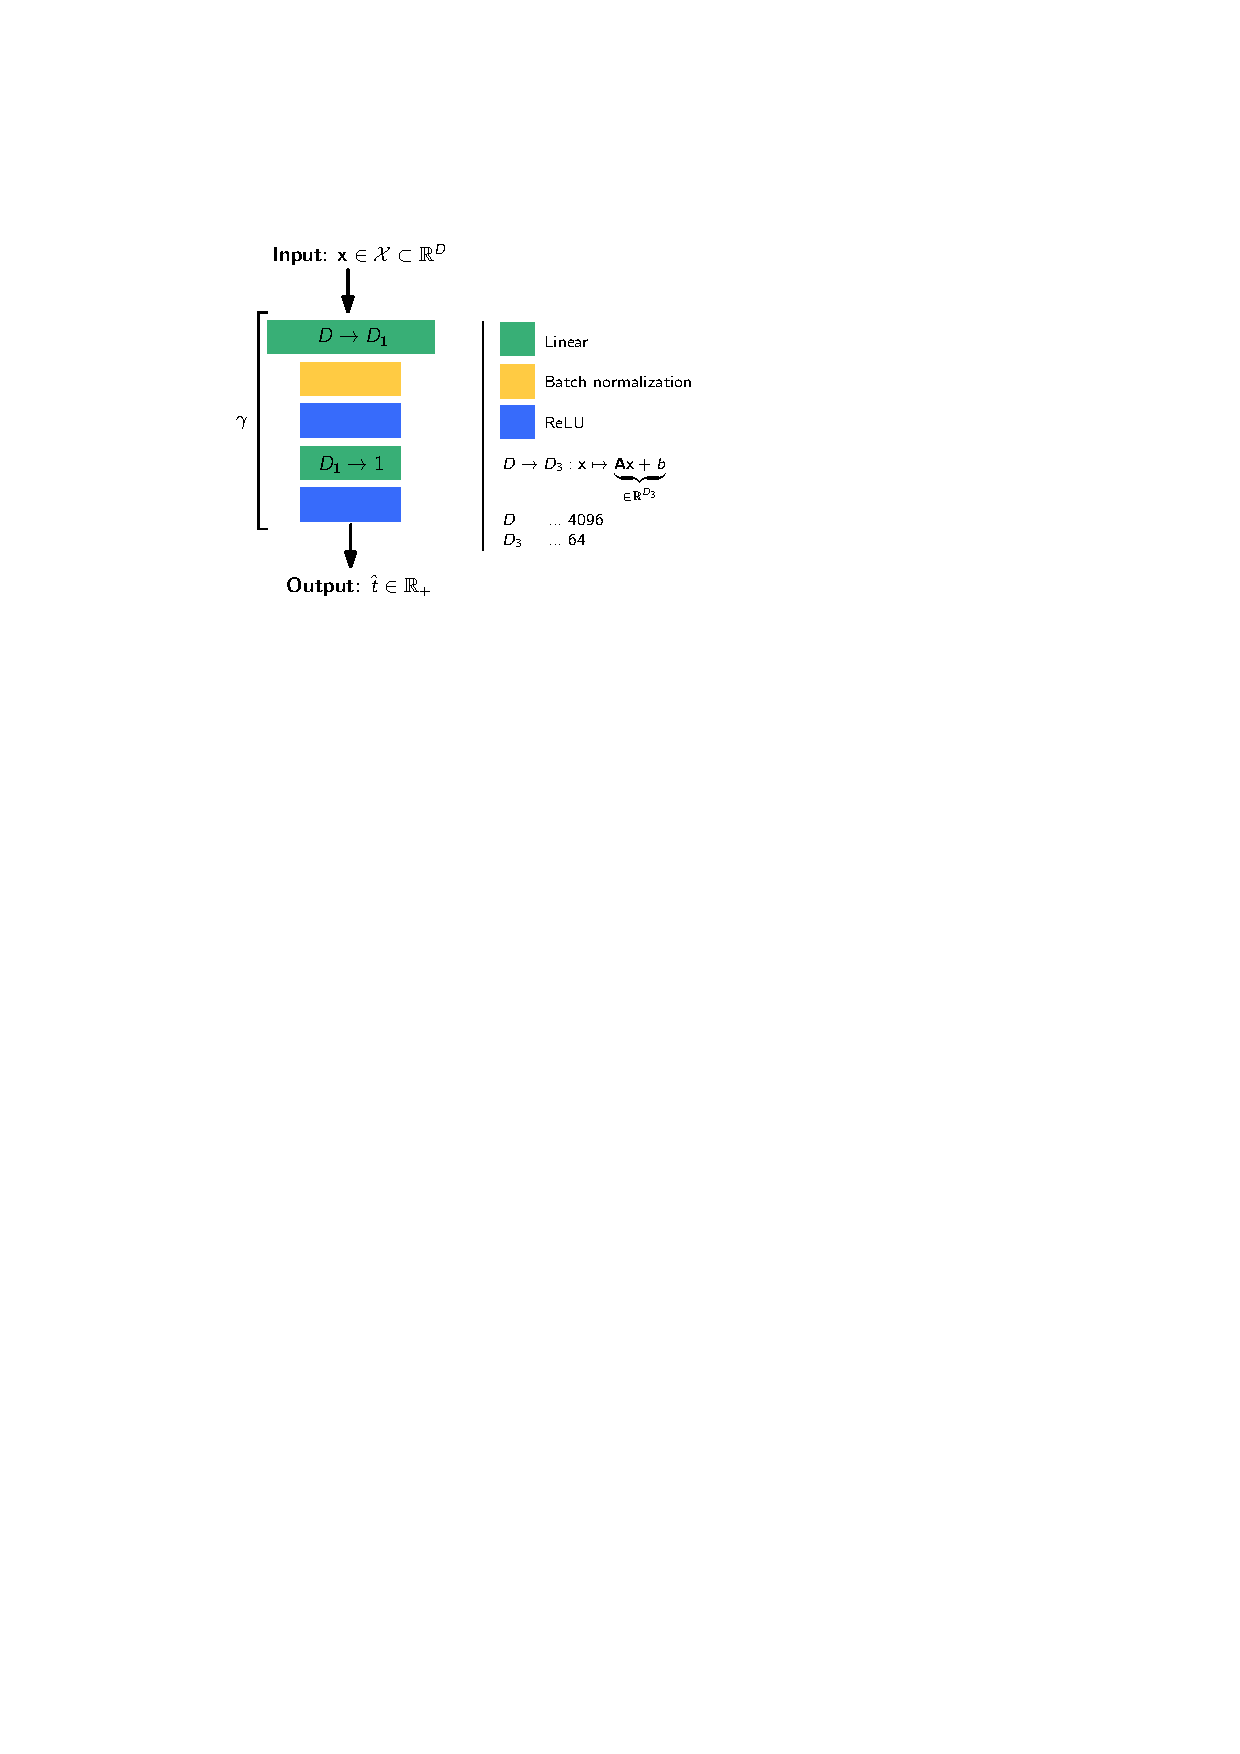
\includegraphics[scale=0.85]{figures/COR}}
\caption{Architecture of the attribute regressor $\gamma$. \label{fig:COR}}
\end{figure}

\vskip0.5ex
\noindent
\textbf{Learning.} The attribute regressor can easily
be trained from a collection of $N$ training tuples $
\{(\mathbf{x}_i,s_i)\}_{i=1}^N$. We remark that for 
this part of the architecture, we do not need any binning 
of the attribute range.

\subsection{Feature regression}
\label{subsection:aug}

To implement $\phi$, we design an encoder-decoder
architecture, reminiscent of a conventional autoencoder \cite{Bengio09a}.
Our objective, however, is not encode and then reconstruct 
the input, but to produce an output that 
resembles a feature descriptor of an object at a 
desired attribute value.

In other words, the \emph{encoder} essentially learns to extract
the essence of features; the \emph{decoder}
then takes the encoding result and decodes it to the desired result. In
general, we can formulate the optimization problem as
\begin{equation}
\min_{\phi \in \mathcal{C}} L(\mathbf{x},t; \phi) = (\gamma(\phi(\mathbf{x}))-t)^2\enspace,
\label{eqn:unconstrained}
\end{equation}
where the minimization is 
over a suitable class of functions $\mathcal{C}$. Notably, when 
implementing $\phi$ as an encoder-decoder network with an 
appended (pre-trained) attribute predictor (see Fig.~\ref{fig:EDN})
and loss $(\gamma(\phi(\mathbf{x}))-t)^2$, we have little control 
over the decoding results in the sense that we cannot guarantee 
that the \emph{identity} of the input is preserved. This means
that features from a particular class of objects might map to 
features that are no longer recognizable as
this class, as the encoder-decoder will \emph{only} learn to ``fool'' the 
attribute predictor $\gamma$.
For that reason, we add a \emph{regularizer} to the objective
of Eq.~\eqref{eqn:unconstrained}, \ie, we require that the 
decoding result needs to be close, \eg, in the $L_2$ norm, to the
input. This changes the optimization problem to
\begin{equation}
\min_{\phi \in \mathcal{C}} L(\mathbf{x},t; \phi) = \underbrace{(\gamma(\phi(\mathbf{x}))-t)^2}_\text{Target mismatch} + 
\lambda \underbrace{\| \phi(\mathbf{x}) - \mathbf{x} \|^2}_{\text{Regularizer}}
\enspace.
\label{eqn:constrained}
\end{equation}
Interpreted differently, this resembles the loss of an autoencoder 
network with an added \emph{target attribute mismatch} term. 
The encoder-decoder network that implements the function class $\mathcal{C}$ 
to learn $\phi$ is shown Fig.~\ref{fig:EDN}. 
The core building block is a combination of a linear layer, 
batch normalization, ELU \cite{Clevert16a}, followed by dropout 
\cite{Srivastava14a}. After the final linear
layer, we add one ReLU layer to enforce $\hat{\mathbf{x}} \in \mathbb{R}^D_+$.

\begin{figure}
\centering{
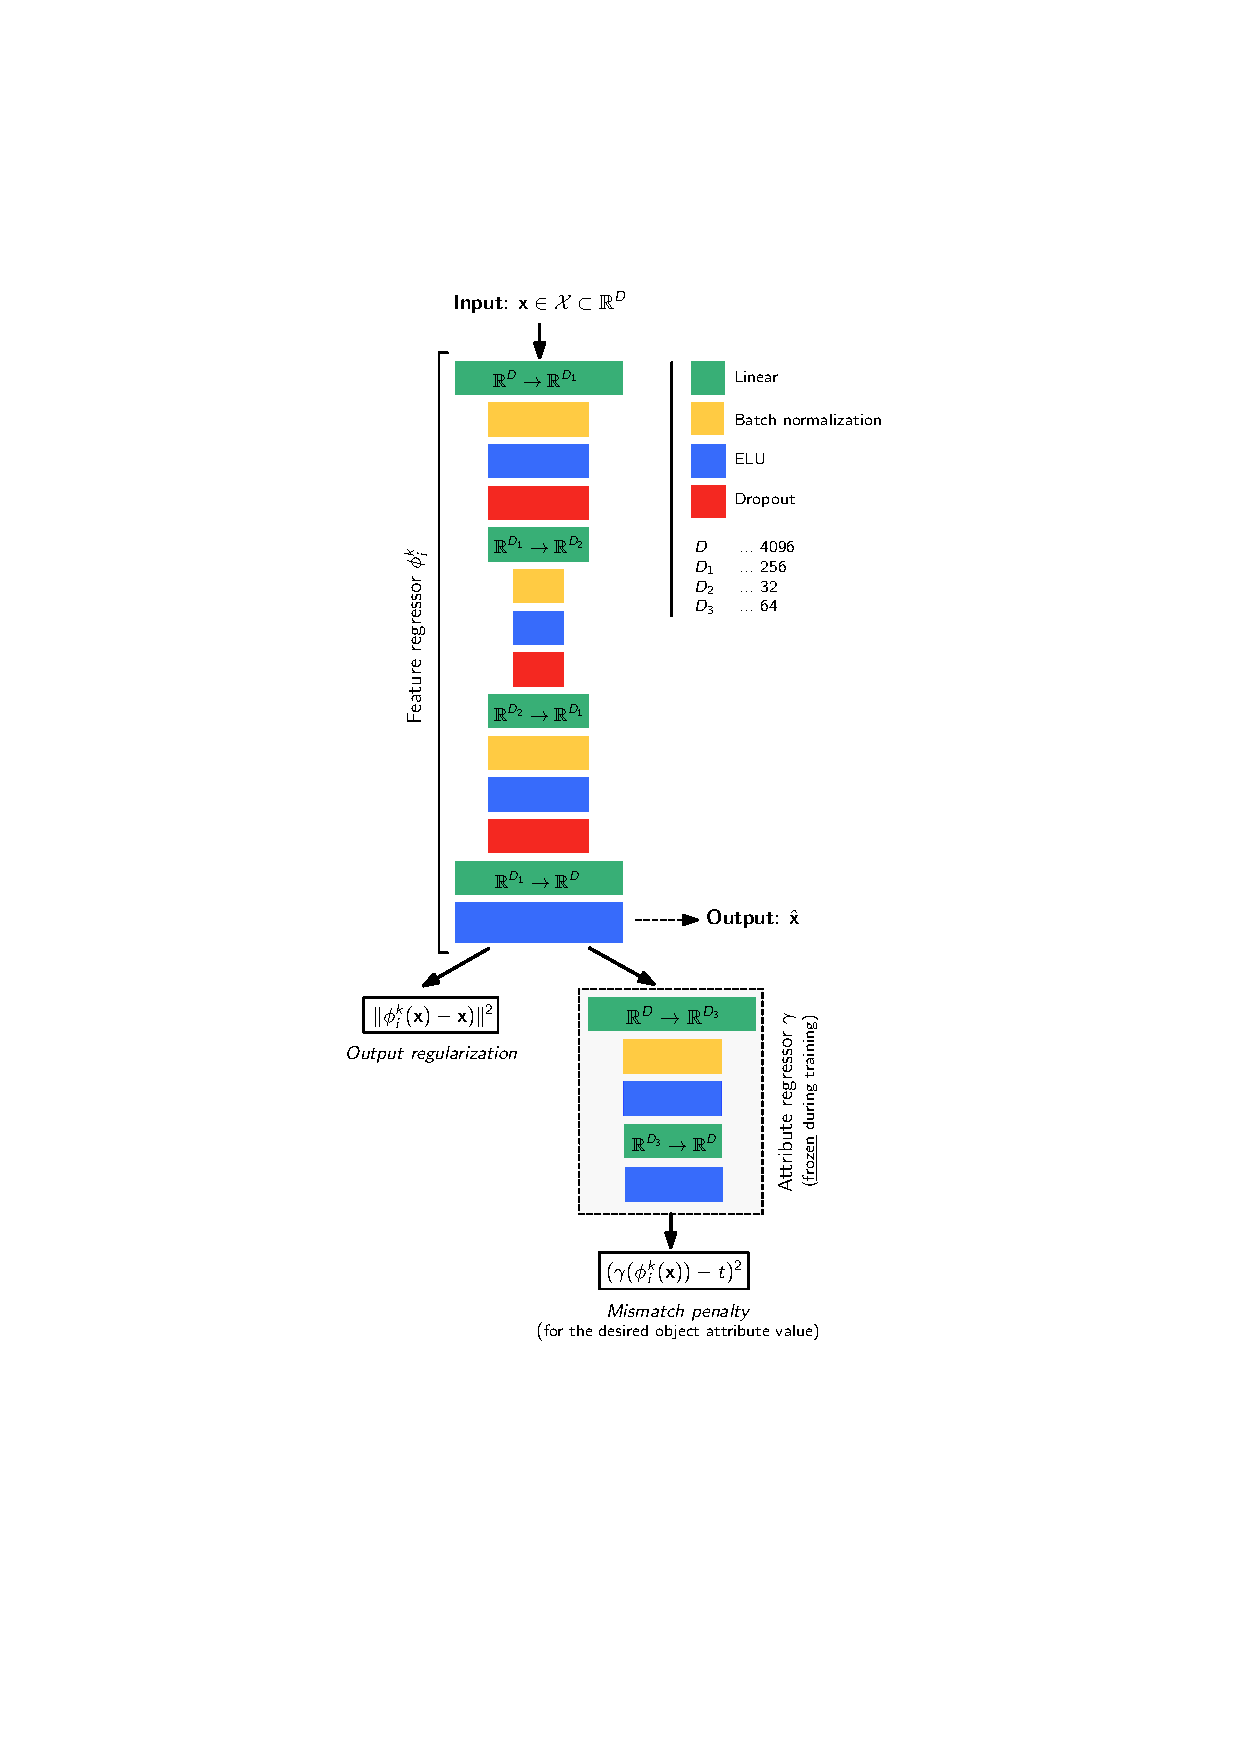
\includegraphics[scale=0.85]{figures/EDN}}
\caption{Illustration of the proposed encoder-decoder network for AGA.
During \emph{training}, the attribute regressor $\gamma$ is appended to
the network, whereas, for \emph{testing} (\ie, feature synthesis) 
this part is removed.
\label{fig:EDN}}
\end{figure}

\vskip1ex
\noindent
\textbf{Learning.} Training the encoder-decoder network of Fig.~\ref{fig:EDN}
first requires a pre-trained attribute regressor $\gamma$ for each given 
attribute $A \in \mathcal{A}$. During training, this
attribute regressor is appended to the network and its 
weights are frozen. Hence, only the encoder-decoder weights
are updated. To train one $\phi_i^k$ for each interval $[l_i,h_i]$ and
target attribute value $t_k$, we partition
the training data from the external corpus into subsets $\mathcal{S}_i$, 
such that $\forall (\mathbf{x}_n,s_n) \in \mathcal{S}_i: s_n \in [l_i,h_i]$. 
Each $\phi_i^k$ is then learned by using only those data tuples. We
note that, since training is done in feature space $\mathcal{X}$, we 
have no convolutional layers and consequently training is 
computationally cheap. For testing, the attribute regressor 
is removed and only the trained encoder-decoder network is used
to synthesize features.

\section{Experiments}
\label{section:experiments}

We first discuss the generation of adequate training data for the 
encoder-decoder network, then evaluate every component of our architecture 
separately and eventually demonstrate its utility on the problem of 
one-shot object recognition in a transfer learning setting.

\vskip1ex
\noindent
\textbf{Dataset.} We use the SUN {RGB-D} dataset from 
Song \etal \cite{Song15a}. This dataset contains 10335 
RGB images with depth maps, as well as detailed 
annotations for more than 1000 objects in the form of 
2D and 3D bounding boxes.
In our setup, we will use object depth and pose as our
object attributes, \ie, $\mathcal{A} = \{\texttt{Depth}, 
\texttt{Pose}\}$. For each ground-truth 2D bounding box 
of an object, we use the depth value at its centroid. Pose
information is computed from the 3D bounding box of 
each object and refers to the rotation of the 3D bounding
box along the $z$-axis. In all experiments, we use the first
5335 images as our \emph{external database}, \ie, the database
for which we assume availability of attribute annotations.
The remaining 5000 images are used for testing; more details
are given in the specific experiments.

\begin{figure}
\centering{
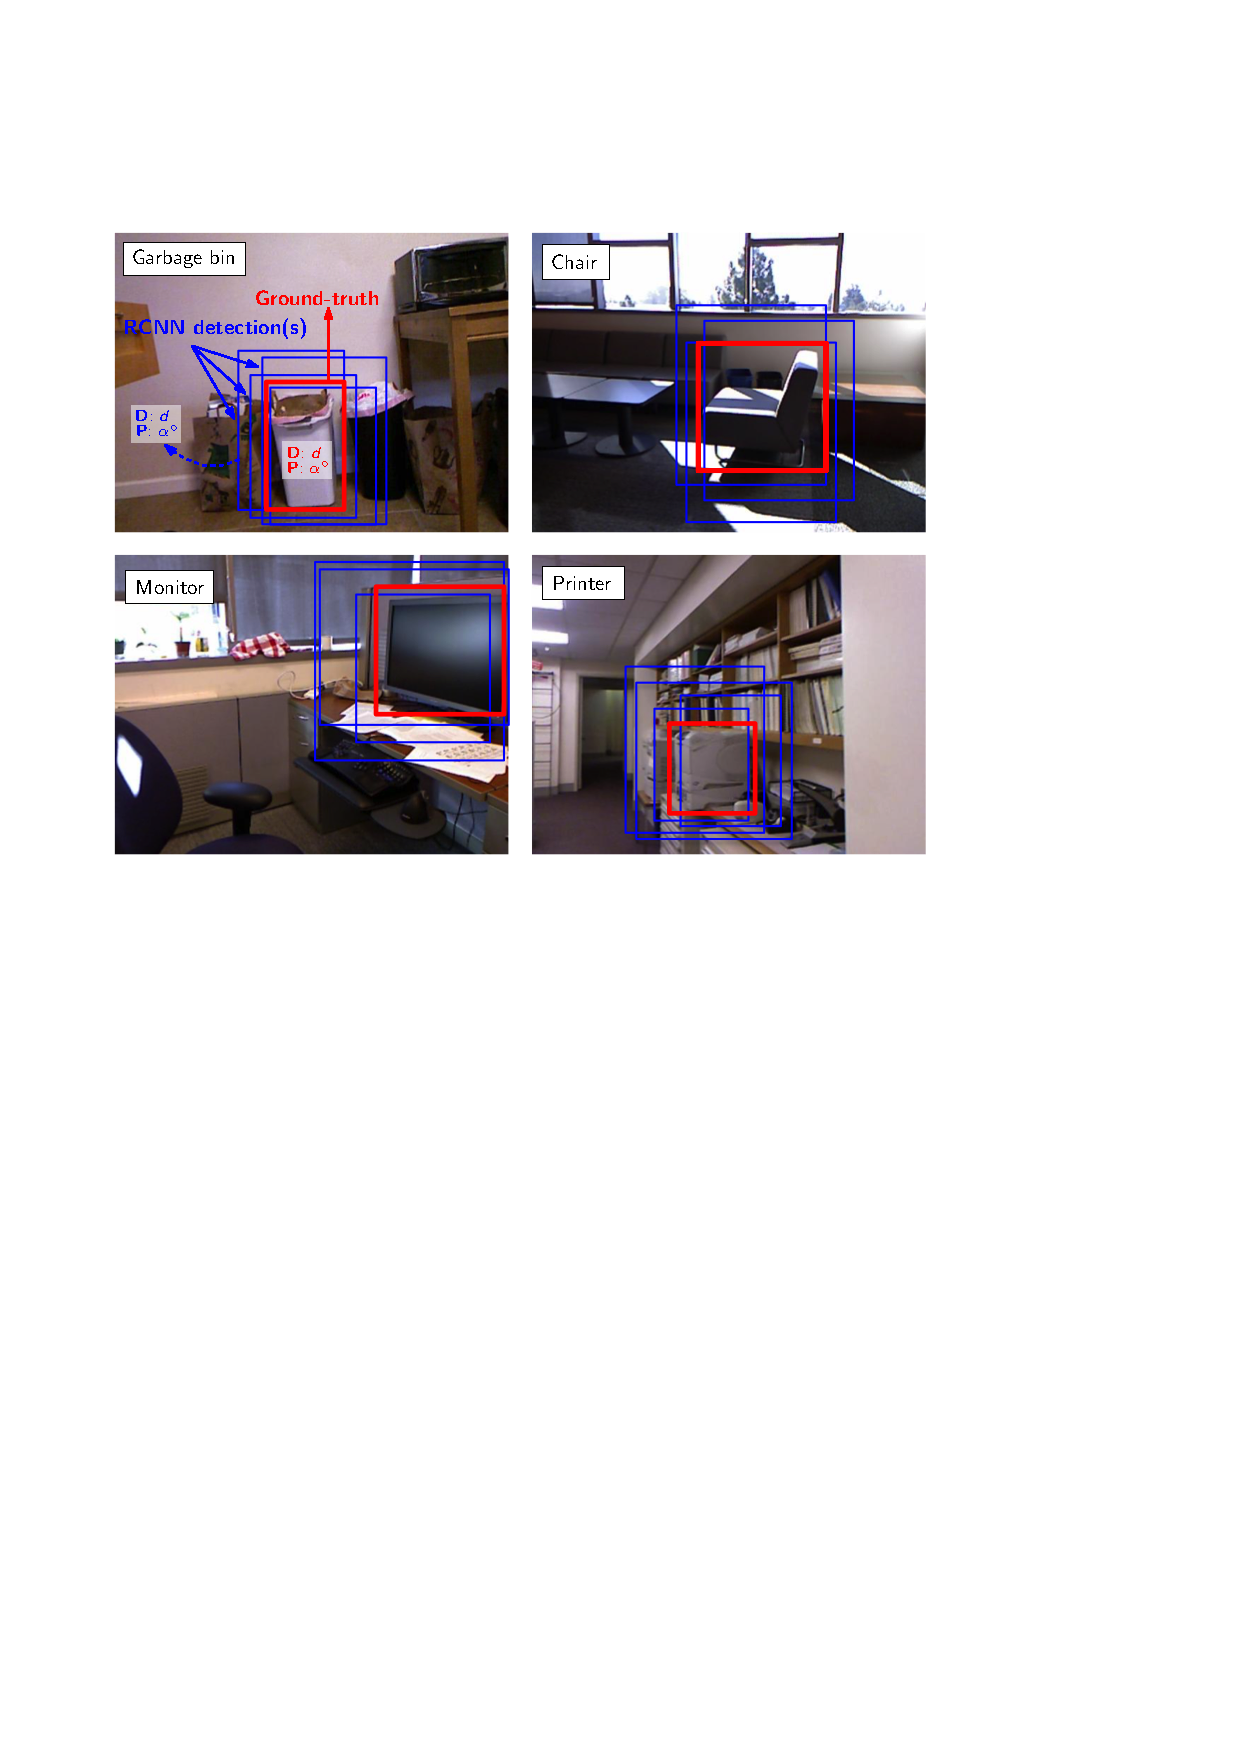
\includegraphics[width=\columnwidth]{figures/TrainingDataIPE}}
\caption{Illustration of \emph{training data generation}. \emph{First}, we keep Fast-RCNN \cite{Girshick15a} activations 
(AlexNet \texttt{FC7}) of Selective Search \cite{Uijlings13a} bounding boxes that overlap with ground-truth
bounding boxes (IoU$>$ 0.5) to generate a sufficient amount of 
training data. \emph{Second}, attribute values (\ie, depth and pose) of the corresponding 3D ground-truth
bounding boxes are transferred to \emph{each} sufficiently overlapping 
selective search box in 2D.\label{fig:trainingdata}}
\end{figure}

\vskip1ex
\noindent
\textbf{Training data.} Notably, in SUN RGB-D, the
number of instances of each object class are not 
evenly distributed, simply because this dataset was
not specifically designed for object recognition tasks. 
Consequently, images are also not object-centric, meaning 
that there is substantial variation in the location of 
objects, as well as the depth and pose at which they occur. 
This makes it difficult to extract a sufficient 
and balanced number of feature descriptors per object class, 
if we would use the ground-truth bounding boxes only. 
We circumvent this problem, by leveraging the Fast-RCNN detector 
of \cite{Girshick15a} with object proposals generated by Selective
Search \cite{Uijlings13a}. In detail, we fine-tune the ImageNet 
model used in \cite{Girshick15a} to SUN RGB-D, using
the same 19 objects as in \cite{Song15a}. We then run 
the detector on all images from our training split and 
keep all bounding boxes with detection scores $>0.7$
and a sufficient overlap (measured by the IoU $>$0.5) 
with the 2D ground-truth bounding boxes.
The associated RCNN activations (at the \texttt{FC7} layer) 
are then used as our features $\mathbf{x}$. Each 
bounding box proposal that remains after overlap and 
score thresholding is annotated by the attribute information 
of the corresponding ground-truth bounding box in 3D. 
As this strategy generates a larger number of descriptors 
(compared to the number of ground-truth bounding
boxes), we can evenly balance the training data in the sense
that we can select an equal number of detections per object
class for training (1) the attribute regressor and (2) the 
encoder-decoder network. Training data generation is illustrated
in Fig.~\ref{fig:trainingdata} on four example images and 
four object classes.

\vskip1ex
\noindent
\textbf{Implementation.} The attribute regressor and 
the encoder-decoder network are implemented in \texttt{Torch}.
All models are trained using \texttt{Adam} \cite{Kingma15a}. 
For the attribute regressor, we train for 30 epochs with a
batch size of 300 and a learning rate of 
$0.001$. The encoder-decoder network also trained for 30
epochs with the same learning rate, but with a batch
size of 128. The dropout probability during training is set to 
$0.25$. No dropout is used for testing. For our classification
experiments, we use a linear C-SVM, as implemented in
\texttt{liblinear} \cite{Fan08a}.
On a Linux system, running
Ubuntu 16.04, with 128 GB of memory and one NVIDIA 
Titan X, training one model (\ie, one $\phi_i^k$) takes 
$\approx 30$ seconds. The relatively low demand on 
computational resources highlights the advantage of 
augmentation in feature space, as no convolutional layers
need to be trained. All trained models are available
at \url{AnonymousURL}.

\subsection{Attribute regression}
\label{subsection:EvalCovariateRegression}

In principle, we have the choice of two training strategies
for the attribute regressor(s). \emph{First}, we could 
train \emph{object-specific} regressors 
$\gamma_c, c \in \{1,\ldots, |\mathcal{C}|\}$, \ie, one regressor
for each object class. This would, however, prevent us from 
using the regressor(s) in a transfer-learning setting, since we
cannot assume knowledge about the object classes that appear in
the target dataset. An alternative, \emph{second} 
strategy is to train \emph{object-agnostic} regressors 
using features from all objects classes together. While 
we will use the object-agnostic model in all subsequent
experiments, we evaluate both strategies to order assess 
the potential loss in prediction performance in the 
object-agnostic setting. 

\begin{table}[t!]
\small
\centering{
\begin{tabular}{rcccc}
\hline
\multirow{ 2}{*}{\textbf{Object}} & \multicolumn{2}{c}{\textbf{D} (MAE [m])}  & \multicolumn{2}{c}{\textbf{P} (MAE [deg])}\\
& per-object & agnostic  & per-object & agnostic \\
\hline
bathtub 	& 0.31 & 1.05 & 36.02 & 108.17\\ 
bed 		& 0.40 & 0.30 & 44.51 & 70.51\\ 
           bookshelf & 0.64 & 0.45 & 50.61 & 95.44 \\ 
                 box & 0.49 & 0.59 & 29.69 & 59.37\\ 
               chair & 0.40 & 0.31 & 37.82 & 53.08 \\ 
             counter & 0.51 & 1.45 & 43.81 & 13.47 \\ 
                desk & 0.39 & 0.36& 48.24 & 47.07 \\ 
                door & 0.41 & 2.03 & 45.62 & 51.84\\ 
             dresser & 0.27 & 0.44 & 65.42 & 63.82\\ 
         garbage bin & 0.34 & 0.32 & 45.93 & 54.43\\ 
                lamp & 0.40 & 1.04 & 30.51 & 132.49\\ 
             monitor & 0.27 & 0.26 & 28.90 & 69.48\\ 
         night stand & 0.53 & 0.85& 28.19 & 99.40 \\ 
              pillow & 0.39 & 0.46 & 34.93 & 73.19\\ 
                sink & 0.17 & 0.20& 60.04 & 59.43 \\ 
                sofa & 0.41 & 0.33& 32.25 & 51.51  \\ 
               table & 0.39 & 0.30 & 41.52 & 50.60\\ 
                  tv & 0.47 & 0.75& 32.33 & 61.77  \\ 
              toilet & 0.24 & 0.23 & 21.58 & 50.89\\ 
		\hline
              \end{tabular}}
\caption{\label{table:maeCOR} Median-Absolute-Error (MAE), for depth / pose, 
of the attribute regressor, evaluated on \emph{19 objects} from \cite{Song15a}.
In our setup, the pose estimation error quantifies the error in predicting a
rotation around the $z$-axis. \textbf{D} indicates \texttt{Depth}, \textbf{P} indicates
\texttt{Pose}.}
\end{table}

Table~\ref{table:maeCOR} lists the median-absolute-error (MAE) of
depth (in [m]) and pose (in [deg]) prediction per object, evaluated 
on instances of 19 object classes extracted from the testing 
portion of SUN RGB-D. As we can see, training in an 
object-specific manner leads to a lower MAE for most objects, both 
for depth and pose. This is not surprising, since the training data 
is more specialized to each particular object, which essentially 
amounts to solving simpler sub-problems. However, in many cases, 
especially for depth, the object-agnostic regressor performs on par, 
except for object classes with fewer training samples (\ie, lamp, door, etc.). 
We also remark that, in general, pose estimation from 2D data is
a substantially harder problem then depth estimation.

\subsection{Feature regression}
\label{subsection:EvalFeatureRegression}

In this section, we assess the performance of the feature regressor(s) 
$\phi_i^k$, \ie, the part of our architecture from Fig.~\ref{fig:EDN} that 
is used to generate synthetic features.

In all experiments, we use an overlapping sliding window to bin
the range of each attribute $A \in \mathcal{A}$ into $T$ 
intervals $[l_i,h_i]$. In case of \texttt{Depth}, we set $[l_0,h_0] = [0,1]$ 
and shift each interval by $0.5$ meter, in case of \texttt{Pose}, we 
set $[l_0,h_0] = [0^\circ,45^\circ]$ and shift by $25^\circ$. 
We generate as many intervals as needed to cover the 
full range of the attribute values in the training data.
The bin-width and step size were set as to ensure a roughly
equal number of associated features in each bin.
For augmentation, we choose $0.5, 1, \ldots, \max(\texttt{Depth})$ as
target attribute values for \texttt{Depth} and  
$45^\circ, 70^\circ,\ldots, 180^\circ$ for \texttt{Pose}. 
This setup results in 11 target values for 
\texttt{Depth} and 7 for \texttt{Pose}. 

\vskip0.5ex
We use two separate evaluation metrics to assess the performance of
$\phi_i^k$. \emph{First}, we are interested in \emph{how well} the feature
regressor can generate features that correspond to the desired attribute
target values. To accomplish this, we run each synthetic feature $\hat{\mathbf{x}}$ through
the attribute predictor and assess the MAE, \ie, $|\gamma(\hat{\mathbf{x}}) -t|$, 
over all attribute targets $t$; Table~\ref{table:ednnonseen} lists the average 
MAE, per object, for (1) features from object classes that were \emph{seen} 
in the training data and (2) features from objects that we have never seen 
before. As wee can see from Table \ref{table:ednnonseen}, MAE's for 
seen and unseen objects are similar, indicating that the encoder-decoder 
has learned to synthesize features, such that $\gamma(\hat{\mathbf{x}}) 
\approx t$.

\vskip0.5ex
\emph{Second}, we are interested in how much synthesized features
differ from original features. While we cannot guarantee an identity
preserving mapping, ``closeness'' to the original features can serve
as a surrogate measure of this desired property.
While, in principle, we could simply evaluate $\|\phi_i^k(\mathbf{x})-\mathbf{x}\|^2$, 
the $L_2$ norm is hard to interpret. Instead, we suggest to compute the 
Pearson correlation coefficient $\rho$ between each original feature and 
its synthesized variants, \ie, 
$\rho(\mathbf{x},\phi_i^k(\mathbf{x}))$. As $\rho$ ranges from $[-1,1]$, 
high values indicate a strong linear relationship to the original features.
Results are reported in Table~\ref{table:ednnonseen}. Contrary to the 
results for MAE, we observe that $\rho$, when averaged over all objects, 
is higher for objects that appeared in the training data. This decrease in
correlation, however, is relatively small. 
 
\begin{table}[t!]
\small
\centering{
\begin{tabular}{cr|cccc}
\hline
& \textbf{Object} & $\rho$ & \textbf{D} (MAE)  & $\rho$ & \textbf{P} (MAE)    \\ \hline
\multirow{19}{*}{\begin{sideways}\textit{Seen} objects, see Table~\ref{table:maeCOR} \end{sideways}} 
&bathtub 		& 0.76 & 0.13 & 0.72 & 6.51\\ 
&bed 		& 0.81 & 0.10 & 0.81 & 4.45 \\ 
&bookshelf 	& 0.80 & 0.09 & 0.80 & 4.90 \\ 
&box 		& 0.73 & 0.11 & 0.75 & 5.32 \\ 
&chair 		& 0.71 & 0.10 & 0.73 & 4.10 \\ 
&counter 		& 0.75 & 0.10 & 0.77 & 5.28\\ 
&desk 		& 0.74 & 0.10 & 0.75 & 4.30 \\ 
&door 		& 0.66 & 0.13 & 0.66 & 6.11 \\ 
&dresser 		& 0.78 & 0.10 & 0.77 & 5.29 \\ 
&garbage bin 	& 0.75 & 0.10 & 0.77 & 4.17 \\ 
&lamp 		& 0.80 & 0.09 & 0.80 & 4.72 \\ 
&monitor 		& 0.82 & 0.09 & 0.82 & 4.25\\ 
&night stand 	& 0.79 & 0.10 & 0.79 & 5.17\\ 
&pillow 		& 0.79 & 0.11 & 0.81 & 4.71 \\ 
&sink 		& 0.75 & 0.11 & 0.75 & 5.33\\ 
&sofa 		& 0.77 & 0.10 & 0.79 & 4.81\\ 
&table 		& 0.73 & 0.10 & 0.75 & 4.53\\ 
&tv 			& 0.78 & 0.11 & 0.76 & 4.69\\ 
&toilet 		& 0.79 & 0.10 & 0.79 & 4.79 \\ \hline
& $\varnothing$ &  \cellcolor{black!10}{\textbf{0.76}} & \cellcolor{black!10}{\textbf{0.11}} & \cellcolor{black!10}{\textbf{0.77}} & \cellcolor{black!10}{\textbf{4.91}} \\
\hline
\multirow{10}{*}{ \begin{sideways}\textit{Unseen} objects \end{sideways} } 
&picture 		& 0.66 & 0.13 & 0.67 & 5.87 \\ 
&ottoman 		& 0.69 & 0.13 & 0.71 & 5.16 \\ 
&whiteboard 	& 0.66 & 0.16 & 0.67 & 6.09 \\ 
&fridge 		& 0.68 & 0.13 & 0.69 & 5.44  \\ 
&counter 		& 0.75 & 0.10 & 0.77 & 5.30\\ 
&books 		& 0.73 & 0.11 & 0.75 & 5.43\\ 
&stove 		& 0.70 & 0.11 & 0.72 & 5.67\\ 
&cabinet 		& 0.73 & 0.11 & 0.73 & 5.52 \\ 
&printer 		& 0.72 & 0.11 & 0.74 & 5.15 \\ 
&computer 		& 0.82 & 0.09 & 0.82 & 4.27 \\ \hline
& $\varnothing$ &  \cellcolor{black!10}{\textbf{0.71}} & \cellcolor{black!10}{\textbf{0.12}} & \cellcolor{black!10}{\textbf{0.73}} &\cellcolor{black!10}{\textbf{5.38}} \\
\hline
\end{tabular}}
\caption{\label{table:ednnonseen} Assessment of $\phi_i^k$ with
respect to (1) Pearson correlation $\rho$ of \emph{synthesized} and 
\emph{original} features and (2) mean MAE of predicted
attribute strengths of synthesized features, $\gamma(\phi_i^k(\mathbf{x}))$,  
with respect to the target attribute values $t$. \textbf{D} indicates
\texttt{Depth}-augmentated features (MAE in [m]); \textbf{P} indicates \texttt{Pose}-augmented
features (MAE in [deg]).}
\end{table}

In summary, we conclude that $\phi_i^k$ can be used on feature descriptors
from object classes that have \emph{not} appeared in the training corpus. 
This enables us to test $\phi_i^k$ in transfer learning setups, 
as we will see in the one-shot experiments of Sec.~\ref{subsection:one-shot}.

\subsection{One-shot object recognition}
\label{subsection:one-shot}

Finally, we demonstrate the utility of our approach on
the problem of one-shot object recognition in a transfer
learning setup. Specifically, we aim to learn attribute-guided 
augmenters $\phi_i^k$ from instances of object classes
that are available in an external, annotated database (in 
our case, SUN RGB-D). We denote this collection of object 
classes as our \emph{source classes} $\mathcal{S}$. 
Given one instance from a collection of a completely different 
object classes, denoted as the \emph{target classes} 
$\mathcal{T}$, we aim to train a discriminant classifier 
$C$ on $\mathcal{T}$, \ie, $C: \mathcal{X} \rightarrow \{1,\ldots,|\mathcal{T}|\}$. 
Hence, in this setting,  $\mathcal{S} \cap \mathcal{T} =
\emptyset$. Note that no attribute annotations for instances 
of object classes in $\mathcal{T}$ are available. 
This can be considered a variant of 
transfer learning, since we transfer knowledge from 
object classes in $\mathcal{S}$ to instances of object
classes in $\mathcal{T}$, \emph{without} any prior knowledge 
about $\mathcal{T}$, except for the single training instances.

\vskip1ex
\noindent
\textbf{Setup.} To evaluate performance on one-shot object 
recognition for \emph{unseen} object classes, we adhere
to the following setup: First, we randomly select two 
collections of 10 object classes to assess the quality
of AGA on different sets of unseen objects. We ensure
that each object class has at least 100 samples in the 
testing split of SUN RGB-D and that no object class in
in $\mathcal{S}$. This guarantees (1) that we have never seen
the image, nor (2) the object category during training.
Since, SUN RGB-D does not have object-centric images, we 
use the ground-truth bounding boxes to obtain the actual 
object crops. This allows us to tease out the actual benefit of 
augmentation without having to deal confounding factors such 
as background noise. The two sets of object classes are denoted 
$\mathcal{T}_1$\footnote{$\mathcal{T}_1$ = \{picture, whiteboard, fridge, counter, books, stove, cabinet, printer, computer, ottoman\}}
and $\mathcal{T}_2$\footnote{$\mathcal{T}_2$ = 
\{mug, telephone, bowl, bottle, scanner, microwave, coffee table, recycle bin, cart, bench\}}. 
We additionally compile a third set of target classes 
$\mathcal{T}_3 = \mathcal{T}_1 \cup \mathcal{T}_2$ and
remark that $\mathcal{T}_1 \cap \mathcal{T}_2 = \emptyset$. 
Consequently, we have two 10-class problems and one 20-class 
problem. For each object image in $\mathcal{T}_i$, we
then collect RCNN \texttt{FC7} features. 

\vskip1ex
As a \emph{Baseline} comparison, we train a linear C-SVM
(with $L_1$-normalized features) 
using only the single instances of each object class in 
$\mathcal{T}_i$. Exactly the same parameter settings of 
the linear SVM, but then used train on the single instances + 
features synthesized by our approach. We repeat the 
selection of one-shot instances 500 times and report
the average recognition accuray. 

\vskip0.5ex
\noindent
\textit{Remark.} Notably, the design of this experiment is somewhat 
similar to \cite[Section 4.3.]{Peng15a}, with the exception 
that we (1) \emph{do not} detect objects, (2) augmentation
is performed in feature space and (3) no 
object-specific information is available. The latter is 
important, since \cite{Peng15a} assumes the existence of 
3D CAD models for objects in $\mathcal{T}$ from which 
synthetic images are generated. In our case, augmentation
does not require any a-priori information about the objects
in the set of target classes.

\vskip1ex
\noindent
\textbf{Results.} Table~\ref{table:oneshot} lists the classification accuracy
for different sets of one-shot training data. \emph{First}, using original
one-shot instances augmented by \texttt{Depth}-guided features (+\textbf{D}); 
\emph{second}, using original features + \texttt{Pose}-guided features 
(+\textbf{D}) and \emph{third}, a combination of the former (+\textbf{D}, \textbf{P});
In general, we observe that adding AGA synthesized features improves 
recognition accuracy over the \emph{Baseline} in all cases. For \texttt{Depth}-augmented
features, gains range from 3-5 percentage points, for \texttt{Pose}-augmented 
features, gains range from 2-4 percentage points on average. We attribute
this effect to the difficuly in predicting object pose from 2D data, an can
be seen from Table~\ref{table:maeCOR}. Nevertheless, in both augmentation settings, 
the gains are statistically significant (\wrt the \emph{Baseline}), as evaluated by a Wilcoxn rank sum test
for equal medians \cite{Gibbons2011a} at $5\%$ significance (indicated by '\checkmark' 
in Table~\ref{table:maeCOR}). Notably, adding \texttt{Depth}- and 
\texttt{Pose}-augmented features to the original one-shot features achieves
the greatest improvement in recognition accuracy, ranging from 4-6 percentage
points, as illustrated in Fig.~\ref{fig:bestoneshot}. This indicates that
information from depth and pose is complementary and allows for better 
coverage of the feature space.
\begin{table}
\begin{tabular}{rcccc}
\hline
& \multirow{2}{*}{\textbf{Baseline}} & \multicolumn{3}{c}{\textbf{AGA} (Ours)}\\
& 						     &  +\textbf{D} & +\textbf{P} &  \textbf{+D}, \textbf{P} \\
\hline
$\mathcal{T}_1$ (10)  	& 33.74	
					&  \cellcolor{green!30}{38.84~\checkmark} 
					&  \cellcolor{green!05}{36.01~\checkmark} 
					&  \cellcolor{green!60}{39.12~\checkmark}\\
$\mathcal{T}_2$ (10) 	& 23.76  	
					&  \cellcolor{green!30}{28.95~\checkmark}
					&  \cellcolor{green!05}{27.01~\checkmark}
					&  \cellcolor{green!60}{30.13~\checkmark}\\
$\mathcal{T}_3$ (20) 	& 22.84	
					&  \cellcolor{green!30}{25.84~\checkmark}
					& \cellcolor{green!05}{24.35~\checkmark}
					&  \cellcolor{green!60}{26.91~\checkmark} \\ 
					\hline
%$\mathcal{S}$ (19) 		& 
%					& 
%					& 
%					& \\
%\hline
\multicolumn{5}{l}{\footnotesize AGA$ \ldots$ Attribute-Guided Augmentation} \\
%\multicolumn{5}{l}{\footnotesize +\textbf{D}$ \ldots$ with \texttt{Depth}} \\
%\multicolumn{5}{l}{\footnotesize +\textbf{D}$ \ldots$ with \texttt{Pose}} \\
%\multicolumn{5}{l}{\footnotesize +\textbf{D},\textbf{P}$ \ldots$ with \texttt{Depth} and \texttt{Pose}} \\
\end{tabular}
\caption{\label{table:oneshot} \emph{Recognition accuracies} (averaged over 500 runs
of randomly selecting one-shot samples) for three one-shot object recognition problems.
The number in parentheses next to $\mathcal{T}_i$ indicates the number of classes.
A '\checkmark' indicates that the result is statistically different (at 5\% significance) 
from the \emph{Baseline} result. +\textbf{D} indicates adding \texttt{Depth}-augmented 
features to the one-shot instances; +\textbf{P} indicates addition of \texttt{Pose}-augmented features
and +\textbf{D}, \textbf{P} denotes adding a combination of \texttt{Depth}-/\texttt{Pose}-augmented 
features.}
\end{table}



\begin{figure}
\centering{
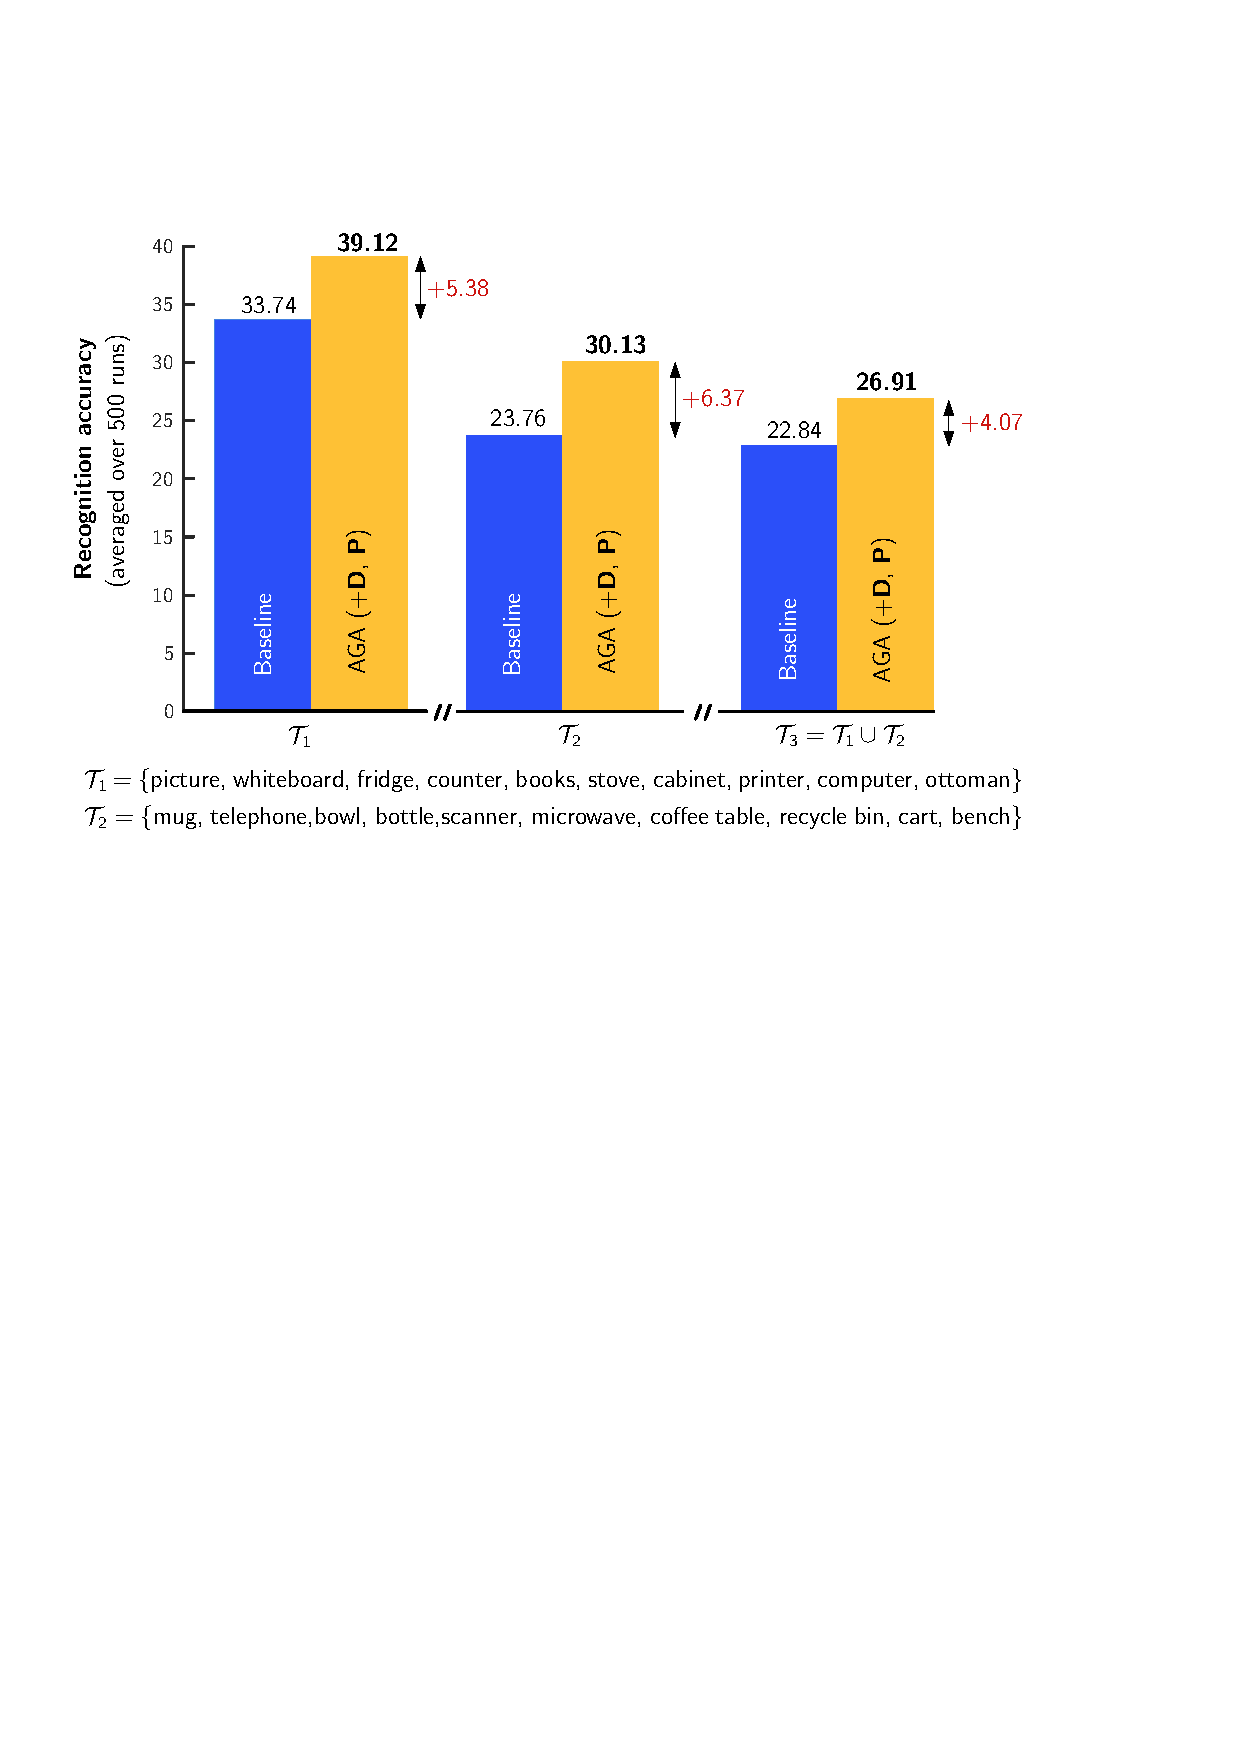
\includegraphics[width=0.99\columnwidth]{figures/OneShotBar}}
\caption{\label{fig:bestoneshot} Comparison of the \textit{Baseline} 
classifier \vs the \emph{best} (\cf Table~\ref{table:oneshot}) one-shot recognition results obtained by AGA, 
over three different sets $\mathcal{T}_i$ of (unseen) object classes. }
\end{figure}

\section{Discussion}
\label{section:discussion}

We presented an approach towards attribute-guided 
augmentation of data in feature space. Our experiments
show that object attributes, such as pose and depth, are
beneficial in the context of one-shot recognition, \ie,
an extreme case of limited training data (apart from 
zero-shot scenarios). While we do use bounding boxes 
to extract object crops from SUN RGB-D, this is only 
done to clearly tease out the effect of augmentation. 
In principle, as our encoder-decoder network is trained
in an \emph{object-agnostic} manner, no external knowledge 
about the target classes is required. 

As SUN RGB-D data exhibits high variability in the range 
of both attributes, augmentation along these dimensions can 
indeed help for classifier training. However, when variability
is constrained, \eg, under controlled acquisition 
settings, the gains may be less apparent. As our approach 
is not limited to depth or pose, augmentation with respect
to other object attributes would be required.

While, training the encoder-decoder network requires 
a pretrained attribute regressor, our results show 
that even in case of mediocre performance of this component 
(\eg, pose prediction), synthesized features can still 
supply useful information to the learning process. 

Several aspects are interesting for future work. \emph{First},
replacing the attribute regressor for pose with a specifically
tailored component, will potentially improve learning of the
augmentation function(s) $\phi_i^k$ and consequently lead to
more realistic synthetic examples. \emph{Second}, we conjecture
that as additional data with object attributes becomes available, 
the encoder-decoder can leverage more diverse samples and 
thus better model changes in the attribute values. 
\emph{Third}, other recognition tasks, \eg, scene recognition,
might equally benefit from AGA, particularly when representations
of scenes are built on top of detected objects, as in \cite{Dixit16a}
for instance.





{\small
\bibliographystyle{ieee}
\bibliography{egbib,halucination}
}

\end{document}
